\documentclass{article}
\usepackage{graphicx}
\usepackage{amsmath}
\usepackage{amssymb}
\usepackage{amsfonts}
\usepackage{graphicx}
\usepackage{float}

\title{MEMAD-T03}
\author{ALEJANDRO ZARATE MACIAS}
\date{8 de Septiembre 2025}

\begin{document}

\maketitle

% ========================================
% INTRODUCCIÓN
% ========================================
\section*{Introducción}
Para la tarea de esta semana se busca trabajar distintos problemas enfocados en el uso de gradientes y su aplicación en métodos de optimización. El objetivo es poner en práctica lo aprendido en los videos proporcionados como material de estudio, así como en los libros sugeridos para el curso. Todo esto con el fin de aplicar:

\begin{itemize}
    \item Propiedades de convexidad.
    \item Teorema de Taylor.
    \item Gradientes: dirección, tamaño de paso, suficiente descenso, etc.
    \item Condiciones de Armijo y Wolfe
    \item Metodos: Newton, Quasi-Newton y Steepest Descent (descenso mas pronunciado)
\end{itemize}
% ========================================
% SECCIÓN 1
% ========================================
\section{Problema 1}

\subsection{Enunciado}
Supóngase que $f(\mathbf{x}) = \mathbf{x}^T Q \mathbf{x}$, donde $Q \in \mathbb{R}^{n \times n}$, $Q \geq 0$, $Q = Q^T$. Demuestre que $f(\mathbf{x})$ es convexa $\forall \, \mathbf{x} \in \mathbb{R}^n$.

\subsection{Metodología}

Para demostrar la convexidad de $f(\mathbf{x})$, utilizaremos el criterio de la matriz hessiana. Una función es convexa si y solo si su matriz hessiana es semidefinida positiva. Por ende, se deben de realizar los siguientes pasos:
\begin{enumerate}
    \item Calcular el gradiente de $f(\mathbf{x})$.
    \item Calcular la matriz hessiana $\nabla^2 f(\mathbf{x})$.
    \item Demostrar que la hessiana es semidefinida positiva utilizando las propiedades dadas de $Q$.
\end{enumerate}

\subsection{Resultados}
\setcounter{equation}{0}

Comenzamos calculando el gradiente de $f(\mathbf{x}) = \mathbf{x}^T Q \mathbf{x}$.
Para una función cuadrática de la forma $\mathbf{x}^T Q \mathbf{x}$, el gradiente está dado por:
\begin{align}
\nabla f(\mathbf{x}) = (Q + Q^T)\mathbf{x}
\end{align}

Dado que $Q = Q^T$ (la matriz es simétrica), tenemos:
\begin{align}
\nabla f(\mathbf{x}) &= (Q + Q)\mathbf{x} \\
&= 2Q\mathbf{x}
\end{align}

Ahora calculamos la matriz hessiana. La hessiana es la matriz de segundas derivadas parciales:
\begin{align}
\nabla^2 f(\mathbf{x}) &= \frac{\partial}{\partial \mathbf{x}}(\nabla f(\mathbf{x})) \\
&= \frac{\partial}{\partial \mathbf{x}}(2Q\mathbf{x}) \\
&= 2Q
\end{align}

Para que $f(\mathbf{x})$ sea convexa, necesitamos que $\nabla^2 f(\mathbf{x}) \geq 0$ (semidefinida positiva).
Dado que $\nabla^2 f(\mathbf{x}) = 2Q$ y sabemos por hipótesis que $Q \geq 0$ (semidefinida positiva), entonces se confirma que:

\begin{equation*}
    f(\mathbf{x}) = \mathbf{x}^T Q \mathbf{x} \quad \text{Es convexa} \quad \forall \, \mathbf{x} \in \mathbb{R}^n
\end{equation*}

\subsection{Discusión}

El resultado demuestra que la convexidad de $f(\mathbf{x}) = \mathbf{x}^T Q \mathbf{x}$ está directamente relacionada con las propiedades de la matriz $Q$. La clave está en que:

\begin{itemize}
    \item La matriz hessiana resulta ser constante: $\nabla^2 f(\mathbf{x}) = 2Q$
    \item Como $Q \geq 0$ por hipótesis, multiplicar por el escalar positivo 2 preserva la propiedad semidefinida positiva
    \item Al ser la hessiana semidefinida positiva en todo punto, la función es convexa globalmente
\end{itemize}

Este resultado es fundamental en optimización, ya que las funciones cuadráticas con matrices semidefinidas positivas aparecen frecuentemente en problemas de optimización convexa.

\subsection{Conclusión}

Se ha demostrado que $f(\mathbf{x}) = \mathbf{x}^T Q \mathbf{x}$ es convexa para toda $\mathbf{x} \in \mathbb{R}^n$ cuando $Q \geq 0$ y $Q = Q^T$. La demostración se basa en que la matriz hessiana $\nabla^2 f(\mathbf{x}) = 2Q$ es semidefinida positiva, lo cual es una condición suficiente para la convexidad. 


% ========================================
% SECCIÓN 2
% ========================================
\section{Problema 2}

\subsection{Enunciado}
Sea $A \in \mathbb{R}^{n \times n}$, $A = A^T$. Considere  
\begin{align*}
    B = A + \alpha \mathbb{I},
\end{align*}
donde $\mathbb{I} \in \mathbb{R}^{n \times n}$ denota la matriz identidad y $\alpha \in \mathbb{R}^{+}$. Demuestre que $B > 0$ para valores suficientemente grandes de $\alpha$.

\subsection{Metodología}

Para demostrar que $B$ es definida positiva para valores suficientemente grandes de $\alpha$, se pueden utilizar las propiedades de los valores propios:
\begin{enumerate}
    \item Analizar los valores propios de $A$ al ser simétrica.
    \item Determinar cómo afecta la adición de $\alpha \mathbb{I}$ a los valores propios.
    \item Encontrar el valor mínimo de $\alpha$ que garantice que todos los valores propios de $B$ sean positivos.
\end{enumerate}

\subsection{Resultados}
\setcounter{equation}{0}

Sea $A$ una matriz simétrica, por el teorema espectral, se puede escribir como:
\begin{align}
A = Q \Lambda Q^T
\end{align}

donde $Q$ es una matriz ortogonal y $\Lambda = \text{diag}(\lambda_1, \lambda_2, \ldots, \lambda_n)$. Además, podemos reescribir a $\mathbb{I}$ como $QQ^T$ (por las propiedades de la matriz identidad). Cuando formamos $B = A + \alpha \mathbb{I}$, obtenemos:

\begin{align}
B &= A + \alpha \mathbb{I} \\
&= Q \Lambda Q^T + \alpha QQ^T \\
&= Q(\Lambda + \alpha \mathbb{I})Q^T \\
&= Q \text{diag}(\lambda_1 + \alpha, \lambda_2 + \alpha, \ldots, \lambda_n + \alpha) Q^T
\end{align}

Por lo tanto, los valores propios de $B$ son:
\begin{align}
\mu_i = \lambda_i + \alpha, \quad i = 1, 2, \ldots, n
\end{align}

Para que $B$ sea definida positiva ($B > 0$), todos sus valores propios deben ser estrictamente positivos:
\begin{align}
\lambda_i + \alpha > 0 \quad \forall \, i = 1, 2, \ldots, n
\end{align}

Sea $\lambda_{\min} = \min\{\lambda_1, \lambda_2, \ldots, \lambda_n\}$ el menor valor propio de $A$. Entonces:
\begin{align}
\alpha > -\lambda_{\min}
\end{align}

Lo que garantiza que $B > 0$.

\subsection{Discusión}

El resultado muestra que siempre es posible hacer que una matriz simétrica sea definida positiva agregando un múltiplo suficientemente grande de la matriz identidad. Esto es posible porque la adición de $\alpha \mathbb{I}$ desplaza todos los valores propios por la misma cantidad $\alpha$, preservando los vectores propios.

\subsection{Conclusión}

Se ha demostrado que para cualquier matriz simétrica $A$, la matriz $B = A + \alpha \mathbb{I}$ es definida positiva cuando $\alpha > -\lambda_{\min}$, donde $\lambda_{\min}$ es el menor valor propio de $A$. Esta técnica es fundamental en métodos de optimización para regularizar matrices hessianas.

% ========================================
% SECCIÓN 3
% ========================================
\section{Problema 3}

\subsection{Enunciado}
Escriba un script en Python para generar una matriz simétrica aleatoria $A \in (-0.5, 0.5)^{10 \times 10}$. Use la idea del Problema 2 para encontrar un valor adecuado de $\alpha$ y construir $B$ tal que $B > 0$. Explique por qué la ``estructura interna'' de ambas matrices $A$ y $B$ permanece igual al inspeccionar su espectro.

\subsection{Metodología}

\subsection{Resultados}
\setcounter{equation}{0}

\subsection{Discusión}

\subsection{Conclusión}

% ========================================
% SECCIÓN 4
% ========================================
\section{Problema 4}

\subsection{Enunciado}
Explique por qué la idea del Problema 2 falla si $A \neq A^T$.

\subsection{Metodología}

Para explicar por qué la técnica falla con matrices no simétricas, se debe analizar:
\begin{enumerate}
    \item Las diferencias en las propiedades espectrales entre matrices simétricas y no simétricas.
    \item Cómo la condición de definida positiva se relaciona con la simetría.
    \item Proporcionar un ejemplo específico que lo pruebe.
\end{enumerate}

\subsection{Resultados}
\setcounter{equation}{0}

La técnica del Problema 2 falla cuando $A \neq A^T$ por una razón simple: el concepto de matriz "definida positiva" solo se aplica a matrices simétricas.

Cuando $A$ no es simétrica, $B = A + \alpha \mathbb{I}$ tampoco será simétrica. Aunque se pueda hacer que $\mathbf{x}^T B \mathbf{x} > 0$, esto no da las propiedades que se necesitan.

\textbf{Ejemplo:}
\begin{align}
A = \begin{pmatrix}
0 & 1 \\
-1 & 0
\end{pmatrix}, \quad B = \begin{pmatrix}
\alpha & 1 \\
-1 & \alpha
\end{pmatrix}
\end{align}

Para cualquier vector $\mathbf{x} = (x_1, x_2)^T$:
\begin{align}
\mathbf{x}^T B \mathbf{x} = \alpha(x_1^2 + x_2^2)
\end{align}

Aunque esto es positivo para $\alpha > 0$, la matriz $B$ sigue sin ser simétrica. 

El problema es que sin simetría:
\begin{itemize}
    \item No podemos garantizar valores propios reales
    \item La descomposición espectral no funciona igual
    \item Las funciones cuadráticas asociadas pueden no ser convexas
\end{itemize}

\subsection{Discusión}

En resumen, la técnica falla porque necesitamos simetría para tener control sobre los valores propios. Sin simetría, agregar $\alpha \mathbb{I}$ no nos garantiza que la matriz resultante tenga las propiedades que buscamos en optimización.

\subsection{Conclusión}

La idea del Problema 2 no funciona para matrices no simétricas porque el concepto de "definida positiva" requiere simetría. Sin esta propiedad, perdemos las garantías necesarias para optimización convexa.

% ========================================
% SECCIÓN NOTAS
% ========================================
\section*{Importante}
\setcounter{equation}{0}
Para los problemas 5 -- 8 considere las siguientes funciones $f : \mathbb{R}^n \rightarrow \mathbb{R}$:

\begin{itemize}
    \item Función de esfera trasladada:\\
    \begin{align}
        f(\mathbf{x}) = \sum_{i=1}^{n} (x_i - c_i)^2, \quad \text{para un determinado (fijo)} \quad \mathbf{c} \in \mathbb{R}^n.
    \end{align}
    Puede tomarse $\mathbf{c} = (1,1,\dots,1)$, por ejemplo.

    \item Función de Rosenbrock:\\
    \begin{align}
        f(\mathbf{x}) = \sum_{i=1}^{n-1} \Big[ 100(x_{i+1} - x_i^{2})^{2} + (x_i - 1)^{2} \Big].
    \end{align}

    \item Función de Perm $n,\beta$:\\
    \begin{align}
        f(\mathbf{x}) =
        \sum_{i=1}^{n} \left(
            \sum_{j=1}^{n}\,(j^{\,i} + \beta)\left( \left(\frac{x_j}{j}\right)^{i} - 1 \right)
        \right)^{2}, \quad \text{para un determinado (fijo)} \quad \beta \in \mathbb{R}.
    \end{align}
    Puede tomarse $\beta = 1$, por ejemplo.
\end{itemize}
Además, como punto inicial considere $\mathbf{x}_0 = (0.5,0.5,\dots,0.5)$. Asimismo, puede suponerse $n=5$.

% ========================================
% SECCIÓN 5
% ========================================
\section{Problema 5}

\subsection{Enunciado}
Calcule analíticamente $\nabla f(\mathbf{x})$ para las funciones (1)--(3).

\subsection{Metodología}

Para calcular los gradientes analíticamente se procederá función por función:
\begin{enumerate}
    \item Función de esfera trasladada: aplicar la regla de la cadena directamente.
    \item Función de Rosenbrock: usar la regla del producto y la cadena para cada término.
    \item Función de Perm: descomponer las sumas anidadas y aplicar derivación paso a paso.
\end{enumerate}

\subsection{Resultados}
\setcounter{equation}{0}

\textbf{1. Función de esfera trasladada:}
\begin{align}
f(\mathbf{x}) = \sum_{i=1}^{n} (x_i - c_i)^2
\end{align}

Para calcular $\frac{\partial f}{\partial x_j}$:
\begin{align}
\frac{\partial f}{\partial x_j} &= \frac{\partial}{\partial x_j} \sum_{i=1}^{n} (x_i - c_i)^2 \\
&= \sum_{i=1}^{n} \frac{\partial}{\partial x_j} (x_i - c_i)^2 \\
&= 2(x_j - c_j)
\end{align}

Por lo tanto:
\begin{align}
\nabla f(\mathbf{x}) = 2(\mathbf{x} - \mathbf{c})
\end{align}

\textbf{2. Función de Rosenbrock:}
\begin{align}
f(\mathbf{x}) = \sum_{i=1}^{n-1} \Big[ 100(x_{i+1} - x_i^{2})^{2} + (x_i - 1)^{2} \Big]
\end{align}

Para $j = 1$:
\begin{align}
\frac{\partial f}{\partial x_1} &= 100 \cdot 2(x_2 - x_1^2) \cdot (-2x_1) + 2(x_1 - 1) \\
&= -400x_1(x_2 - x_1^2) + 2(x_1 - 1)
\end{align}

Para $1 < j < n-1$:
\begin{align}
\frac{\partial f}{\partial x_j} &= 100 \cdot 2(x_j - x_{j-1}^2) + 100 \cdot 2(x_{j+1} - x_j^2) \cdot (-2x_j) + 2(x_j - 1) \\
&= 200(x_j - x_{j-1}^2) - 400x_j(x_{j+1} - x_j^2) + 2(x_j - 1)
\end{align}

Para $j = n$:
\begin{align}
\frac{\partial f}{\partial x_n} &= 100 \cdot 2(x_n - x_{n-1}^2) \\
&= 200(x_n - x_{n-1}^2)
\end{align}

\textbf{3. Función de Perm $n,\beta$:}
\begin{align}
f(\mathbf{x}) = \sum_{i=1}^{n} \left( \sum_{j=1}^{n}\,(j^{\,i} + \beta)\left( \left(\frac{x_j}{j}\right)^{i} - 1 \right) \right)^{2}
\end{align}

Esta función es más compleja debido a las sumas anidadas. Para simplificar el análisis, definimos:
\begin{align}
S_i = \sum_{j=1}^{n}\,(j^{\,i} + \beta)\left( \left(\frac{x_j}{j}\right)^{i} - 1 \right)
\end{align}

Entonces la función se puede escribir como:
\begin{align}
f(\mathbf{x}) = \sum_{i=1}^{n} S_i^2
\end{align}

Para calcular $\frac{\partial f}{\partial x_k}$, aplicamos la regla de la cadena:
\begin{align}
\frac{\partial f}{\partial x_k} &= \sum_{i=1}^{n} \frac{\partial}{\partial x_k}(S_i^2) = \sum_{i=1}^{n} 2S_i \frac{\partial S_i}{\partial x_k}
\end{align}

Ahora necesitamos calcular $\frac{\partial S_i}{\partial x_k}$. En la suma $S_i$, solo el término con $j = k$ depende de $x_k$:
\begin{align}
\frac{\partial S_i}{\partial x_k} &= \frac{\partial}{\partial x_k}\left[(k^i + \beta)\left( \left(\frac{x_k}{k}\right)^{i} - 1 \right)\right] \\
&= (k^i + \beta) \frac{\partial}{\partial x_k}\left(\frac{x_k}{k}\right)^{i} \\
&= (k^i + \beta) \cdot i \cdot \left(\frac{x_k}{k}\right)^{i-1} \cdot \frac{1}{k} \\
&= (k^i + \beta) \cdot \frac{i}{k} \cdot \left(\frac{x_k}{k}\right)^{i-1}
\end{align}

Sustituyendo de vuelta:
\begin{align}
\frac{\partial f}{\partial x_k} = 2\sum_{i=1}^{n} S_i \cdot (k^i + \beta) \cdot \frac{i}{k} \cdot \left(\frac{x_k}{k}\right)^{i-1}
\end{align}

\textbf{Forma completa del gradiente de la función Perm:}

El $k$-ésimo componente del gradiente es:
\begin{align}
\frac{\partial f}{\partial x_k} = 2\sum_{i=1}^{n} \left[ \sum_{j=1}^{n}\,(j^{\,i} + \beta)\left( \left(\frac{x_j}{j}\right)^{i} - 1 \right) \right] \cdot (k^i + \beta) \cdot \frac{i}{k} \cdot \left(\frac{x_k}{k}\right)^{i-1}
\end{align}

donde $k = 1, 2, \ldots, n$.

\subsection{Discusión}

Los gradientes calculados muestran diferentes niveles de complejidad. La función esfera trasladada tiene el gradiente más simple (lineal), mientras que Rosenbrock y Perm tienen gradientes no lineales más complejos. Esto afectará directamente la velocidad de convergencia de los algoritmos de optimización.

\subsection{Conclusión}

Se han calculado analíticamente los gradientes de las tres funciones. La función esfera trasladada tiene gradiente lineal, Rosenbrock tiene términos cuadráticos y cúbicos, y la función Perm tiene la expresión más compleja con potencias variables dependiendo de los parámetros $i$ y $k$.

% ========================================
% SECCIÓN 6
% ========================================
\section{Problema 6}

\subsection{Enunciado}
Implemente en Python el algoritmo de descenso más pronunciado (SD) para las funciones $ (1)-(3) $. Use un paso de longitud fija y el gradiente analítico. Muestre gráficas del número de iteraciones contra el valor de la función.

\subsection{Metodología}

\subsection{Resultados}
\setcounter{equation}{0}

\subsection{Discusión}

\subsection{Conclusión}

% ========================================
% SECCIÓN 7
% ========================================
\section{Problema 7}

\subsection{Enunciado}
Mejore su script anterior usando un gradiente numérico en lugar del gradiente analítico. A continuación, resuelva el problema de minimización para las funciones (1)-(3) usando el mismo número de iteraciones que antes. Realice una comparación de las soluciones obtenidas con las del Problema 6.


\subsection{Metodología}

\subsection{Resultados}
\setcounter{equation}{0}

\subsection{Discusión}

\subsection{Conclusión}

% ========================================
% SECCIÓN 8
% ========================================
\section{Problema 8}

\subsection{Enunciado}
Mejore aún más su script añadiendo longitudes de paso de tipo decreciente lineal, adaptativa e inteligente (i.e.\ condiciones de Armijo o de Wolfe). Puede usar un gradiente analítico o numérico. Use algunas gráficas para comparar los resultados obtenidos con cada una de las cuatro estrategias de longitud de paso.

\subsection{Metodología}

\subsection{Resultados}
\setcounter{equation}{0}

\subsection{Discusión}

\subsection{Conclusión}

% ========================================
% SECCIÓN 9
% ========================================
\section{Problema 9}

\subsection{Enunciado}
Considere la siguiente función

\begin{align}
    f(x_1, x_2) = 10^{9}x_1^{2} + x_2^{2}. \tag{4}
\end{align}

Considere $\mathbf{x}_0 = (1.5, 1.5)$ como punto inicial. Resuelva el problema de minimización usando su script de $SD$. ¿Cuántas iteraciones necesita su implementación de $SD$ para alcanzar un valor de la función menor que $1e^{-4}$? A continuación, escale las variables de (4). ¿Cuántas iteraciones necesita su implementación de $SD$ para alcanzar un valor menor que $1e^{-4}$ en esta versión escalada de (4)?


\subsection{Metodología}

\subsection{Resultados}
\setcounter{equation}{0}

\subsection{Discusión}

\subsection{Conclusión}

% ========================================
% SECCIÓN 10
% ========================================
\section{Problema 10}

\subsection{Enunciado}
La diferenciación analítica y numérica no son las únicas formas de calcular derivadas. Investigue un poco sobre la diferenciación automática. Luego, considere la función de Himmelblau:

\begin{align}
    f(x,y) = (x^{2} + y - 11)^{2} + (x + y^{2} - 7)^{2}. \tag{5}
\end{align}

Calcule las derivadas parciales de (5) en el punto $(1,-1)$ usando diferenciación automática (dibuje en papel las gráficas correspondientes y muestre su procedimiento). ¿Qué ventajas y desventajas tienen la diferenciación analítica, numérica y automática al compararlas entre sí?

\subsection{Metodología}

Para aplicar diferenciación automática se seguirá el modo directo (forward mode):
\begin{enumerate}
    \item Descomponer la función en operaciones elementales.
    \item Construir el grafo correspondiente.
    \item Evaluar simultáneamente la función y sus derivadas usando la regla de la cadena.
    \item Comparar los tres métodos de diferenciación.
\end{enumerate}

\subsection{Resultados}
\setcounter{equation}{0}

La función de Himmelblau se puede descomponer como:
\begin{align}
f(x,y) = u_1^2 + u_2^2
\end{align}
donde $u_1 = x^2 + y - 11$ y $u_2 = x + y^2 - 7$.

El grafo computacional correspondiente se muestra en la Figura~\ref{fig:grafo_himmelblau}:

\begin{figure}[H]
\centering
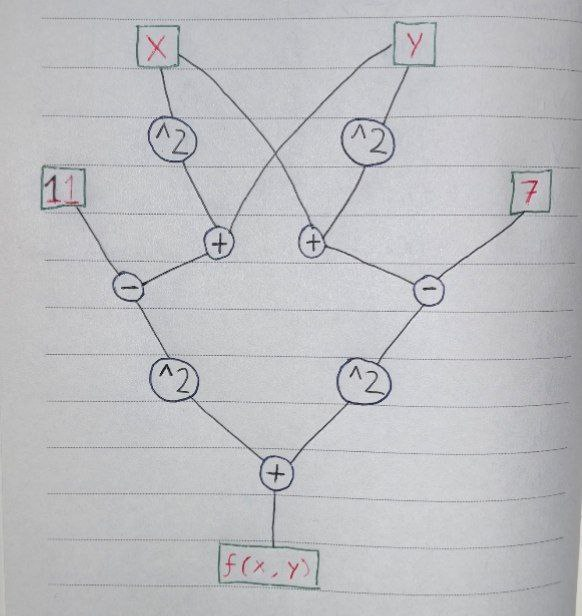
\includegraphics[width=0.5\textwidth]{images/10_autodiff.jpg}
\caption{Grafo computacional para la función de Himmelblau usando diferenciación automática.}
\label{fig:grafo_himmelblau}
\end{figure}

Usando el grafo dibujado, evaluamos en el punto $(1,-1)$:

Para\textbf{ $\frac{\partial f}{\partial x}$:}
Inicializamos con $\dot{x} = 1, \dot{y} = 0$.

\begin{table}[h]
\centering
\begin{tabular}{|l|c|c|l|}
\hline
\textbf{Operación} & \textbf{Valor} & \textbf{Derivada} & \textbf{Cálculo} \\
\hline
$x$ & $1$ & $1$ & Entrada inicial \\
$y$ & $-1$ & $0$ & Entrada inicial \\
\hline
$v_1 = x^2$ & $1$ & $2$ & $\dot{v_1} = 2x\dot{x} = 2(1)(1) = 2$ \\
$v_2 = y^2$ & $1$ & $0$ & $\dot{v_2} = 2y\dot{y} = 2(-1)(0) = 0$ \\
\hline
$v_3 = v_1 + y$ & $0$ & $2$ & $\dot{v_3} = \dot{v_1} + \dot{y} = 2 + 0 = 2$ \\
$v_4 = x + v_2$ & $2$ & $1$ & $\dot{v_4} = \dot{x} + \dot{v_2} = 1 + 0 = 1$ \\
\hline
$v_5 = v_3 - 11$ & $-11$ & $2$ & $\dot{v_5} = \dot{v_3} = 2$ \\
$v_6 = v_4 - 7$ & $-5$ & $1$ & $\dot{v_6} = \dot{v_4} = 1$ \\
\hline
$v_7 = v_5^2$ & $121$ & $-44$ & $\dot{v_7} = 2v_5\dot{v_5} = 2(-11)(2) = -44$ \\
$v_8 = v_6^2$ & $25$ & $-10$ & $\dot{v_8} = 2v_6\dot{v_6} = 2(-5)(1) = -10$ \\
\hline
$f = v_7 + v_8$ & $146$ & $-54$ & $\dot{f} = \dot{v_7} + \dot{v_8} = -44 + (-10) = -54$ \\
\hline
\end{tabular}
\caption{Evaluación forward para $\frac{\partial f}{\partial x}$ en $(1,-1)$}
\end{table}

Para\textbf{ $\frac{\partial f}{\partial y}$:}
Inicializamos con $\dot{x} = 0, \dot{y} = 1$.

\begin{table}[h]
\centering
\begin{tabular}{|l|c|c|l|}
\hline
\textbf{Operación} & \textbf{Valor} & \textbf{Derivada} & \textbf{Cálculo} \\
\hline
$x$ & $1$ & $0$ & Entrada inicial \\
$y$ & $-1$ & $1$ & Entrada inicial \\
\hline
$v_1 = x^2$ & $1$ & $0$ & $\dot{v_1} = 2x\dot{x} = 2(1)(0) = 0$ \\
$v_2 = y^2$ & $1$ & $-2$ & $\dot{v_2} = 2y\dot{y} = 2(-1)(1) = -2$ \\
\hline
$v_3 = v_1 + y$ & $0$ & $1$ & $\dot{v_3} = \dot{v_1} + \dot{y} = 0 + 1 = 1$ \\
$v_4 = x + v_2$ & $2$ & $-2$ & $\dot{v_4} = \dot{x} + \dot{v_2} = 0 + (-2) = -2$ \\
\hline
$v_5 = v_3 - 11$ & $-11$ & $1$ & $\dot{v_5} = \dot{v_3} = 1$ \\
$v_6 = v_4 - 7$ & $-5$ & $-2$ & $\dot{v_6} = \dot{v_4} = -2$ \\
\hline
$v_7 = v_5^2$ & $121$ & $-22$ & $\dot{v_7} = 2v_5\dot{v_5} = 2(-11)(1) = -22$ \\
$v_8 = v_6^2$ & $25$ & $20$ & $\dot{v_8} = 2v_6\dot{v_6} = 2(-5)(-2) = 20$ \\
\hline
$f = v_7 + v_8$ & $146$ & $-2$ & $\dot{f} = \dot{v_7} + \dot{v_8} = -22 + 20 = -2$ \\
\hline
\end{tabular}
\caption{Evaluación forward para $\frac{\partial f}{\partial y}$ en $(1,-1)$}
\end{table}

Proceso paso a paso:

1. Inicialización\textbf{:} Se establecen las variables de entrada $(x,y) = (1,-1)$ y las semillas direccionales $(\dot{x}, \dot{y})$ según la derivada que se quiera calcular.

2. Operaciones\textbf{ }elementales\textbf{:} Cada operación en el grafo se evalúa propagando tanto el valor como su derivada usando las reglas:
   \begin{itemize}
       \item Potenciación: $\frac{d}{dx}(u^n) = nu^{n-1}\frac{du}{dx}$
       \item Suma: $\frac{d}{dx}(u + v) = \frac{du}{dx} + \frac{dv}{dx}$
       \item Constante: $\frac{d}{dx}(u + c) = \frac{du}{dx}$
   \end{itemize}

3. Propagación\textbf{:} Los valores y derivadas se propagan hacia adelante en el grafo hasta llegar a la función objetivo.

Resultados en $(1,-1)$:
\begin{align}
f(1,-1) &= 146 \\
\frac{\partial f}{\partial x}\bigg|_{(1,-1)} &= -54 \\
\frac{\partial f}{\partial y}\bigg|_{(1,-1)} &= -2
\end{align}

\subsection{Discusión}

\textbf{Comparación de métodos de diferenciación:}

\begin{itemize}
    \item Diferenciación Analítica: 
        \begin{itemize}
            \item Ventajas: Exacta, expresión simbólica, eficiente para evaluaciones múltiples
            \item Desventajas: Requiere derivación manual, propensa a errores, compleja para funciones complicadas
        \end{itemize}
    
    \item Diferenciación Numérica:
        \begin{itemize}
            \item Ventajas: Fácil de implementar, aplicable a cualquier función
            \item Desventajas: Errores de truncamiento y redondeo, inestable numéricamente, costosa computacionalmente
        \end{itemize}
    
    \item Diferenciación Automática:
        \begin{itemize}
            \item Ventajas: Exacta hasta precisión de máquina, automática, eficiente
            \item Desventajas: Requiere software especializado, overhead de memoria en modo reverso
        \end{itemize}
\end{itemize}

\subsection{Conclusión}

La diferenciación automática combina las ventajas de los métodos analítico y numérico: proporciona derivadas exactas sin requerir derivación manual. En el ejemplo de la función de Himmelblau, se obtuvieron las derivadas parciales $\frac{\partial f}{\partial x} = -54$ y $\frac{\partial f}{\partial y} = -2$ en $(1,-1)$ de manera sistemática y precisa usando el grafo computacional.

\end{document}
